\documentclass[twocolumn,astrosymb]{aastex631}

%% The default is a single spaced, 10 point font, single spaced article.
%% There are 5 other style options available via an optional argument. They
%% can be invoked like this:
%%
%% \documentclass[arguments]{aastex631}
%% 
%% where the layout options are:
%%
%%  twocolumn   : two text columns, 10 point font, single spaced article.
%%                This is the most compact and represent the final published
%%                derived PDF copy of the accepted manuscript from the publisher
%%  manuscript  : one text column, 12 point font, double spaced article.
%%  preprint    : one text column, 12 point font, single spaced article.  
%%  preprint2   : two text columns, 12 point font, single spaced article.
%%  modern      : a stylish, single text column, 12 point font, article with
%% 		  wider left and right margins. This uses the Daniel
%% 		  Foreman-Mackey and David Hogg design.
%%  RNAAS       : Supresses an abstract. Originally for RNAAS manuscripts 
%%                but now that abstracts are required this is obsolete for
%%                AAS Journals. Authors might need it for other reasons. DO NOT
%%                use \begin{abstract} and \end{abstract} with this style.
%%
%% Note that you can submit to the AAS Journals in any of these 6 styles.
%%
%% There are other optional arguments one can invoke to allow other stylistic
%% actions. The available options are:
%%
%%   astrosymb    : Loads Astrosymb font and define \astrocommands. 
%%   tighten      : Makes baselineskip slightly smaller, only works with 
%%                  the twocolumn substyle.
%%   times        : uses times font instead of the default
%%   linenumbers  : turn on lineno package.
%%   trackchanges : required to see the revision mark up and print its output
%%   longauthor   : Do not use the more compressed footnote style (default) for 
%%                  the author/collaboration/affiliations. Instead print all
%%                  affiliation information after each name. Creates a much 
%%                  longer author list but may be desirable for short 
%%                  author papers.
%% twocolappendix : make 2 column appendix.
%%   anonymous    : Do not show the authors, affiliations and acknowledgments 
%%                  for dual anonymous review.
%%
%% these can be used in any combination, e.g.
%%
%% \documentclass[twocolumn,linenumbers,trackchanges]{aastex631}
%%
%% AASTeX v6.* now includes \hyperref support. While we have built in specific
%% defaults into the classfile you can manually override them with the
%% \hypersetup command. For example,
%%
%% \hypersetup{linkcolor=red,citecolor=green,filecolor=cyan,urlcolor=magenta}
%%
%% will change the color of the internal links to red, the links to the
%% bibliography to green, the file links to cyan, and the external links to
%% magenta. Additional information on \hyperref options can be found here:
%% https://www.tug.org/applications/hyperref/manual.html#x1-40003
%%
%% Note that in v6.3 "bookmarks" has been changed to "true" in hyperref
%% to improve the accessibility of the compiled pdf file.
%%
%% If you want to create your own macros, you can do so
%% using \newcommand. Your macros should appear before
%% the \begin{document} command.
%%
\newcommand{\vdag}{(v)^\dagger}
\newcommand\aastex{AAS\TeX}
\newcommand\latex{La\TeX}

\newcommand{\code}[1]{\textbf{\texttt{#1}}}
\newcommand{\sersic}{S\'ersic}
\usepackage{CJKutf8}
\usepackage{bm}
\usepackage{appendix}
\usepackage{amsmath,amssymb}

%% Reintroduced the \received and \accepted commands from AASTeX v5.2
\received{\today}
\revised{\today}
\accepted{\today}

\submitjournal{ApJ}

%% alias for citations
\defcitealias{Greco2018}{G18}

% \def\G18{\citetalias{Greco2018}}

\shorttitle{UDGs in MW analogs}
\shortauthors{Li et al.}
%%
%% You can add a light gray and diagonal water-mark to the first page 
%% with this command:
%% \watermark{text}
%% where "text", e.g. DRAFT, is the text to appear.  If the text is 
%% long you can control the water-mark size with:
%% \setwatermarkfontsize{dimension}
%% where dimension is any recognized LaTeX dimension, e.g. pt, in, etc.
%%
%%%%%%%%%%%%%%%%%%%%%%%%%%%%%%%%%%%%%%%%%%%%%%%%%%%%%%%%%%%%%%%%%%%%%%%%%%%%%%%%
\graphicspath{{./}{figures/}}
%% This is the end of the preamble.  Indicate the beginning of the
%% manuscript itself with \begin{document}.

\begin{document}
\begin{CJK*}{UTF8}{gbsn}

\title{Ultra Diffuse Galaxies associated with Milky-Way Analogs}

% \correspondingauthor{Jiaxuan Li}
\author[0000-0001-9592-4190]{Jiaxuan Li (李嘉轩)}
\affiliation{Department of Astrophysical Sciences, 4 Ivy Lane, Princeton University, Princeton, NJ 08544, USA}

\author[0000-0002-5612-3427]{Jenny E. Greene}
\affiliation{Department of Astrophysical Sciences, 4 Ivy Lane, Princeton University, Princeton, NJ 08544, USA}

\author[0000-0003-4970-2874]{Johnny Greco}
\affiliation{Department of Astrophysical Sciences, 4 Ivy Lane, Princeton University, Princeton, NJ 08544, USA}
\affiliation{Center for Cosmology and AstroParticle Physics (CCAPP), The Ohio State University, Columbus, OH 43210, USA}

\author[0000-0003-1385-7591]{Song Huang (黄崧)}
\affiliation{Department of Astrophysical Sciences, 4 Ivy Lane, Princeton University, Princeton, NJ 08544, USA}
\affiliation{Department of Astronomy and Tsinghua Center for Astrophysics, Tsinghua University, Beijing 100084, China}

\author{Peter Melchior}
\affiliation{Department of Astrophysical Sciences, 4 Ivy Lane, Princeton University, Princeton, NJ 08544, USA}
\author{Remy Joseph}
\affiliation{Department of Astrophysical Sciences, 4 Ivy Lane, Princeton University, Princeton, NJ 08544, USA}

%% I'd like to invite Shany?

%% Note that the \and command from previous versions of AASTeX is now
%% depreciated in this version as it is no longer necessary. AASTeX 
%% automatically takes care of all commas and "and"s between authors names.

%% AASTeX 6.31 has the new \collaboration and \nocollaboration commands to
%% provide the collaboration status of a group of authors. These commands 
%% can be used either before or after the list of corresponding authors. The
%% argument for \collaboration is the collaboration identifier. Authors are
%% encouraged to surround collaboration identifiers with ()s. The 
%% \nocollaboration command takes no argument and exists to indicate that
%% the nearby authors are not part of surrounding collaborations.

%% Mark off the abstract in the ``abstract'' environment. 
\begin{abstract}

\end{abstract}

\keywords{Low surface brightness galaxies (940), Dwarf galaxies (416), Galaxy properties (615), Galaxy abundances (574)}


\section{Introduction} \label{sec:intro}

In this work, we use the circularized effective radius $r_{\rm eff}$, defined as the $r_{\rm eff} = r_{\rm eff, sma} \sqrt{b/a}$, where $r_{\rm eff, sma}$ is the effective radius along the semi-major axis of the aligned elliptical isophotes, and $b/a$ is the axis ratio of the isophotes.

We adopt a $\Lambda$CDM cosmology from \citet{Planck15} with $\Omega_{\rm m}= 0.307$ and $H_0 = 67.7\ $km s$^{-1}$ Mpc$^{-1}$. We use the AB system \citep{Oke1983} for magnitudes. The stellar mass used in this work is based on a \citet{Chabrier2003} initial mass function.

\section{Data} \label{sec:data}
\subsection{Hyper Suprime-Camera data}
The Hyper Suprime-Camera Subaru Strategic Program Survey (\citealt{Aihara2018}; hereafter HSC survey)\footnote{\url{https://hsc-release.mtk.nao.ac.jp/doc/}} is an optical imaging survey using the 8.2-m Subaru telescope and the Hyper Suprime-Camera \citep{Miyazaki2012, Miyazaki2018}. The \texttt{Wide} layer is designed to cover $\sim 1000\ \rm{deg}^{2}$ of the sky in five broad bands ($grizy$), reaching a depth of $g=26.6$ mag, $r=26.2$ mag and $i=26.2$ mag ($5\sigma$ point source). HSC data are processed using \code{hscPipe}\footnote{\url{https://hsc.mtk.nao.ac.jp/pipedoc_e/}} \citep{Bosch2018}, which is a customized version of the Large Synoptic Survey Telescope (LSST) pipeline \citep{LSST-pipeline}\footnote{\url{https://pipelines.lsst.io/}}. 

In this work, we use the \code{Wide} layer data from Public Data Release 2 (PDR2, also known as \code{S18A}) of HSC \citealt{Aihara2018}. It covers $\sim 300\ \rm{deg}^2$ in all five bands, which is 1.5 times larger than the dataset analyzed in \citetalias{Greco2018}. One of the key improvements made in \code{S18A} is the sky background subtraction. Compared with previous data releases, \code{S18A} adopted a full focal plane sky subtraction algorithm to overcome the over-subtraction of local sky background around bright objects \citep{Aihara2018,Li2021}. The unprecedented depth and careful sky subtraction makes \code{S18A} an ideal dataset to search for low surface brightness galaxies. 

%HSC \code{S18A} also provides bitmasks indicating bad pixels, cosmic rays, edges of CCDs and pixels with source detection, helping us generate image masks when extracting surface brightness profiles (Section \ref{sec:hsc_methods}). In this paper, we use the \code{WIDE} layer data from \code{S18A} (\code{PDR2}). It covers $\sim 300$ deg$^2$ in all five bands. 

\subsection{NASA-Sloan Atlas}
We use the NASA-Sloan Atlas (NSA \footnote{\url{http://nsatlas.org}}, \citealt{Blanton2005,Blanton2011}) to select galaxies analogous to the Milky Way. NSA is a catalog of parameters of local galaxies derived from the Sloan Digital Sky Survey \citep[SDSS,][]{York2000}. We use the new version of NSA catalog (\code{v1\_0\_1}\footnote{\url{https://www.sdss.org/dr13/manga/manga-target-selection/nsa/}}) which contains about $640,000$ galaxies out to $z < 0.15$. It also includes elliptical Petrosian aperture photometry for galaxies, which is considered to be more reliable than the photometry used in older versions. In this paper, we use the stellar mass derived from the ellpitical Petrosian photometry using \code{kcorrect v4\_2}. The redshifts of galaxies in NSA come from several spectroscopic surveys, gas surveys, or direct distance measurements. 



\section{Methodology}
\subsection{Source Detection}\label{subsec:detection}
\citetalias{Greco2018} performed a search for extended LSBGs in the first $\sim 200$ deg$^2$ of HSC survey. We continued the work in \citetalias{Greco2018} and extended the search to HSC \code{S18A} data which covers $\sim 300\ \rm{deg}^{2}$ and has much better sky subtraction compared to \code{S16A}. We follow the same philosophy of source detection as in \citetalias{Greco2018}, but make several updates to accommodate \code{S18A} data. Below we summarize the main steps of the search and emphasize the updates made to improve the overall completeness and purity. We refer interested readers to \citetalias{Greco2018} for more details. Our source detection pipeline \code{hugs}\footnote{\url{https://github.com/johnnygreco/hugs}} is also publically available.

\begin{enumerate}
    \item \textbf{Bright source removal}. Bright sources and their associated LSB lights can mimic objects of interest and obstruct effective detection of LSBGs. In this step, we replace pixels related to bright sources with sky noise. The bright sources and their diffuse lights are detected by applying a high thresholding and a low thresholding to the image. A diffuse light component is associated with a bright source if more than 15\% of its pixels are above the high threshold. In this way, we generate a footprint of bright sources in the image.
    
    Since the sky subtraction in \code{S18A} is significantly better than in previous data releases, LSB features are well conserved after subtracting the sky. Therefore, it makes more sense to set the thresholding based on surface brightness, instead of a certain sigma value above sky background (as in \citetalias{Greco2018}). We set the high threshold to $\mu_{\rm high} = 22\ \mathrm{mag\ arcsec^{-2}}$ to capture all bright sources above this surface brightness, and the low threshold to $\mu_{\rm low} = 24.5\ \mathrm{mag\ arcsec^{-2}}$ to capture associated diffuse lights. 
    
    %Unlike in \citetalias{Greco2018}, we do not smooth the image prior to thresholding. 
    After this step, there are still a number of small low surface brightness objects, which are typically marginally resolved galaxies or just pixels with high noise fluctuations. We detect and remove them since our main goal is to detect extended LSBGs. We run \code{sep}\footnote{\url{https://sep.readthedocs.io/en/v1.1.x/}} \citep{Barbary2016} on the image cleaned as above. Based on the segmantation map, we generate a mask for sources smaller than $r_{\rm min} = 2\arcsec$. This step reduces the number of blended sources. These values ($\mu_{\rm high},\ \mu_{\rm low},\ r_{\rm min})$ are chosen by trial and error. 

    In the end, we replace pixels within the bright source footprint and small source mask with sky noise. The detection is done in $i$-band, and we use the same mask for all $gri$-bands. This step effectively cleans out objects and features that hinder the detection of LSBGs. 
    
    \item \textbf{Source Extraction}. We use \code{Source Extractor} \citep{Bertin1996} to detect sources on the ``cleaned'' images produced in the previous step. This step remains largely the same as in \citetalias{Greco2018}. The images are convoled with a Gaussian kernel of FWHM=$1\arcsec$ to maximize the contrast. We take a mesh size of $43\arcsec$ (doubles the size used in \citetalias{Greco2018}) to measure the local bacbkground and detect objects that are 0.7$\sigma$ per pixel above the local sky. We also require the object contains at least 100 contiguous pixels to further remove small compact objects. We perform the detection in $g$-band but require all the sources are also detected in $r$-band to exclude possible artifacts. 
    
    \item \textbf{Initial Sample Selection}. In this step, we take the output catalog from the previous step and remove those objects that are not likely to be LSBGs of interest. To be specific, we require objects have $g$-band half-light radius (measured by Source Extractor) larger than $r_{\rm min} = 2.0\arcsec$. We also require the measured colors to satisfy $-0.1 < g-i < 1.4$ and $|(g-r) - 0.7\cdot (g-i)| < 0.4$. %These cuts are the same as in \citetalias{Greco2018}. 
    \textbf{Morphology? Auto-correlation?}
    
    
\end{enumerate}
After these steps, we have an intial sample containing 86,002 LSBG candidates. \textbf{Why we obtain more sources per sqr deg compared with G18? Sky?} Among these objects, there are still a lot of false positives, including galaxy outskirts, tidal features, blended compact sources, etc. Therefore, we perform an extra ``deblending'' step to remove false positives.  

\subsection{Deblending}
A common type of false positive occurs when point-like sources are blended with diffuse lights from background galaxies or LSB outskirts of  stars and galaxies. In order to remove these objects from our sample, we perform non-parametric modeling for  each object using \code{scarlet}\footnote{\url{https://pmelchior.github.io/scarlet/}} \citep{Melchior2018}. \code{scarlet} is a deblending and modeling tool designed for multi-band data. It utilizes the color and morphology information to seperate blended sources. In the following, we briefly summarize how \code{scarlet} works, and we refer intersted readers to \citet{Melchior2018} for more details. In \code{scarlet}, each source in the scene $Y_i$ is described by a morphology matrix $S_i$ and a Spectral Energy Distribution (SED) vector $A_i$. The goal of modeling is to minimize the object function $f \propto \frac{1}{2}||\sum Y_i - P(\sum A_i S_i)||_2^{2}$ under certain constraints, where $P$ is the convolution with PSF. The morphology matrix of each source is limited to be within a bounding box. In this section, we assume that all sources have positive fluxes (positivity constraint) and the light profiles of all sources monotonically decreases from their centers to outskirts (monotonoicity constraint). Although not all galaxies satisfy the monotonicity constraint, it still provides an easy, sparse, and robust way to deblend overlapping sources. We refer to this modeling method as the ``vanilla scarlet''. 

In vanilla scarlet, objects can be modeled with different types of sources, including point source, single-extended source, multi-extended source, compact-extended source, and flat-sky source. The morphology matrix of point source is simply the normalized PSF. For the single-extended source, the morphology matrix follows positivity and monotonicity constraints. The multi-extended source is a combination of two or more single-extended sources, which makes it possible to model more complex structure and color gradient of galaxies. The compact-extended source is a single-extended source initialized using the morphology matrix of a point-source, which encourages the model to be compact. The flat-sky source has uniform color and morphology across the box.

Vanilla scarlet is ideal to identify and remove the false positives in our intial LSBG sample. 

We model LSBG candidates using vanilla scarlet as follows. 

\begin{enumerate}
\item \textbf{Peak detection.} We first generate cutout images with a size of $1\arcmin$ in $griz$-bands for each LSBG candiate. Then we construct a detection image by taking a weighted average of the images in four separate bands. We take the total inverse variance as the weight for each band. This detection image is considered to be deeper than any single band image. 

Next, we detect peaks on the detection image. We first run \code{sep} on the detection image using a detection threshold of 4$\sigma$, a mesh size of 48 pixels ($8\arcsec$), and a kernel size of 3 pixels. This step idenfities relatively extended sources in the detection image. However, there are still faint and compact peaks not detected. Therefore, we apply a wavelet decomposition to the detection image \citep{Starck2015} and only keep high spatial frequency components. Another round of \code{sep} is then ran on this high-frequency image using a detection threshold of 2.5$\sigma$, a mesh size of 24 pixels, and a kernel size of 3 pixels. This step detects many compact sources that are not detected in the previous step. In the end, we combine the two detection catalogs together. 

\item \textbf{Model initialization and optimization}.
The deblending step is designed to deblend sources in the vicinity of the target object. The scene will contain both the target object and all the sources in its vicinity. Therefore, the sources being modeled is determined by how extended the target is. We estimate a bounding box based on the detection image, and include all the peaks inside this box to be modeled.

We use a multi-extended source with two components to model the target object, such that it is capable to capture the details of galaxy structure and color. The source is initialized as follows. We start by convolving the detection image with a circular Gaussian kernel with $\sigma=1.5$ pixels to boost the contrast between the signal and the sky noise \citep[e.g.,][]{Irwin1985,Akhlaghi2015,Greco2018}. After smoothing, the low surface brightness outskirts of target galaxy will become more prominent, which helps intializing the morphology matrix. The smoothed detection image is thresholded using $0.1\sigma$ to remove sky noise, then the morphology matrix $S_i$ of the intial model is determined by constructing a symmetric and monotonic approximation to the region in the detection image around the peak of the target object. The intial SED vector $A_i$ is set to be the color of the image averaged with the spatial weight function $S_i$. As a byproduct of intialization, we get a bounding box which represents the extent of the target object. We also add a flat-sky source to model the local sky around the target. This is helpful for situations where an object overlaps with the LSB outskirts of a bright galaxy.

Then we initialize all the sources inside the bounding box of the target. The extended objects detected in the first detection step are modeled as single-extended sources. For compact objects that are only detected in the second step, we model them as point sources if their FWHM $<$ 5 pixels, otherwise as compact-extended sources. The morphology matrices and SED vectors of these sources are also intialized in the same way as above. 

As mentinoed above, we only model sources within the bounding box of the target. However, scattered lights from nearby bright stars and galaxies could bias the modeling within the bounding box. We match our field with the GAIA catalog and mask out stars outside of the bounding box. Since we have already detected peaks throughout the whole cutout image, we also generate a mask for objects outside the bounding box to reduce the impact of scattered light from bright galaxies. 

As a result of such initialization, we only optimize the object function $f$ defined for sources within the bounding box of the target object. The optimization process uses the adaptive proximal gradient method \citep{Melchior2019}, which is a robust method for optimization with constraints. The model is considered to be converged when the relative changes of parameters are smaller than \code{e\_rel\,=\,2e-4}. Typically convergence is achieved after $\sim 50$ steps of opimization and the whole modeling takes about 40s for each LSBG. 

\textbf{For bright sources? }

\item \textbf{Measurement.}
After running vanilla scarlet, we get non-parametric models of objects within the bounding box of the target. We take out the model of the target galaxy (as shown in Figure \ref{fig:vanilla_scarlet_demo}) and analyze it using \code{statmorph}\footnote{\url{https://statmorph.readthedocs.io/en/latest/}}\citep{statmorph}. The goal of this step is to remove false positives using various morphological and structural diagnostics.

\code{Statmorph} calculates non-parametric morphological and structural parameters, including the half-light radius, concentration-asymmetry-smoothness (CAS) statistics \citep{Conselice2003}, Gini-M20 \citep{Lotz2004}, etc. It takes an image, a segmentation map indicating the footprint of the object, a variance map, and PSF. For our purpose, the image is just the scarlet model convolved with the observed PSF. This image represents the deblended target galaxy. Because there is no contaminants in the deblended model, the segmentation map just covers the whole image. The variance map and PSF are taken from HSC cutouts. We also force the sky level to be zero because sky has already been fit in vanilla scarlet. 

One of the most important diagnostics is the size of the object. Half-light radius is calculated using ellpitical apertures, where the ellipticity $\varepsilon$ is determined by calculating the second moment of the image. We define the circularized half-light radius $r_e$ as the geometrical average of the semi-major and semi-minor axis of the half-light elliptical aperture: $r_e = r_{\rm sma} \sqrt{b/a}$. The total magnitudes are simply calculated by summing up the model in each band, and colors are defined by the difference among apparent magnitudes. Galactic extinction correction is not applied at this point. Two kinds of surface brightnesses are measured. The central surface brightness $\mu_0$ is measured by extrapolating the surface brightness profile to $r\to 0$. We also define the average surface brightness within effective radius as $\mu_{\rm eff} = m - 2.5 \log_{10}(2 \pi r_e^2)$, where $m$ is the total magnitude. 

We also use Gini-M20 and CAS statistics. The Gini coefficient \citep{Abraham2003,Lotz2004} and M20 statistics quantify how concentrated/extended is the flux distribution across the image. The CAS statistics characterize the concentration ($C = 5\log_{10}(r_{80} / r_{20}$), asymmetry, and smoothness of the light distribution of the object. We refer the readers to \citet{statmorph} for more details on their definitions and implementations. The morphological and structural parameters are the same in different bands due to the construction of \code{scarlet} model.


We apply the following cuts:

\begin{itemize}
    \item Color:
    \[0.0 < g-i < 1.2,\ |(g-r) - 0.7\cdot (g-i)| < 0.25\]
    \item Size: \[2 \arcsec < r_e < 12 \arcsec\]
    \item Surface brightness: \[\mu_0(g) > 22.5,\ 23.0 < \mu_{\rm eff}(g) < 27.5,\]
    \item Morphology: 
    \begin{gather*}
        \varepsilon < 0.65,\ 1.8 < C < 3.5,\\
        \mathrm{Gini} < 0.70,\ M_{20} < -1.1,
    \end{gather*}
\end{itemize}


To better guide us on how to use these diagnostics, we visually inspected a subset of LSBG candiates. 

The measured parameters here does not neccesarily represent the truth. We only use them to rule out false positives in a purely empirical way. The half-light radius is often too small because the cookie-cutter effect. 


\begin{figure*}
	\vbox{ 
		%\vskip -10mm
		\centering
		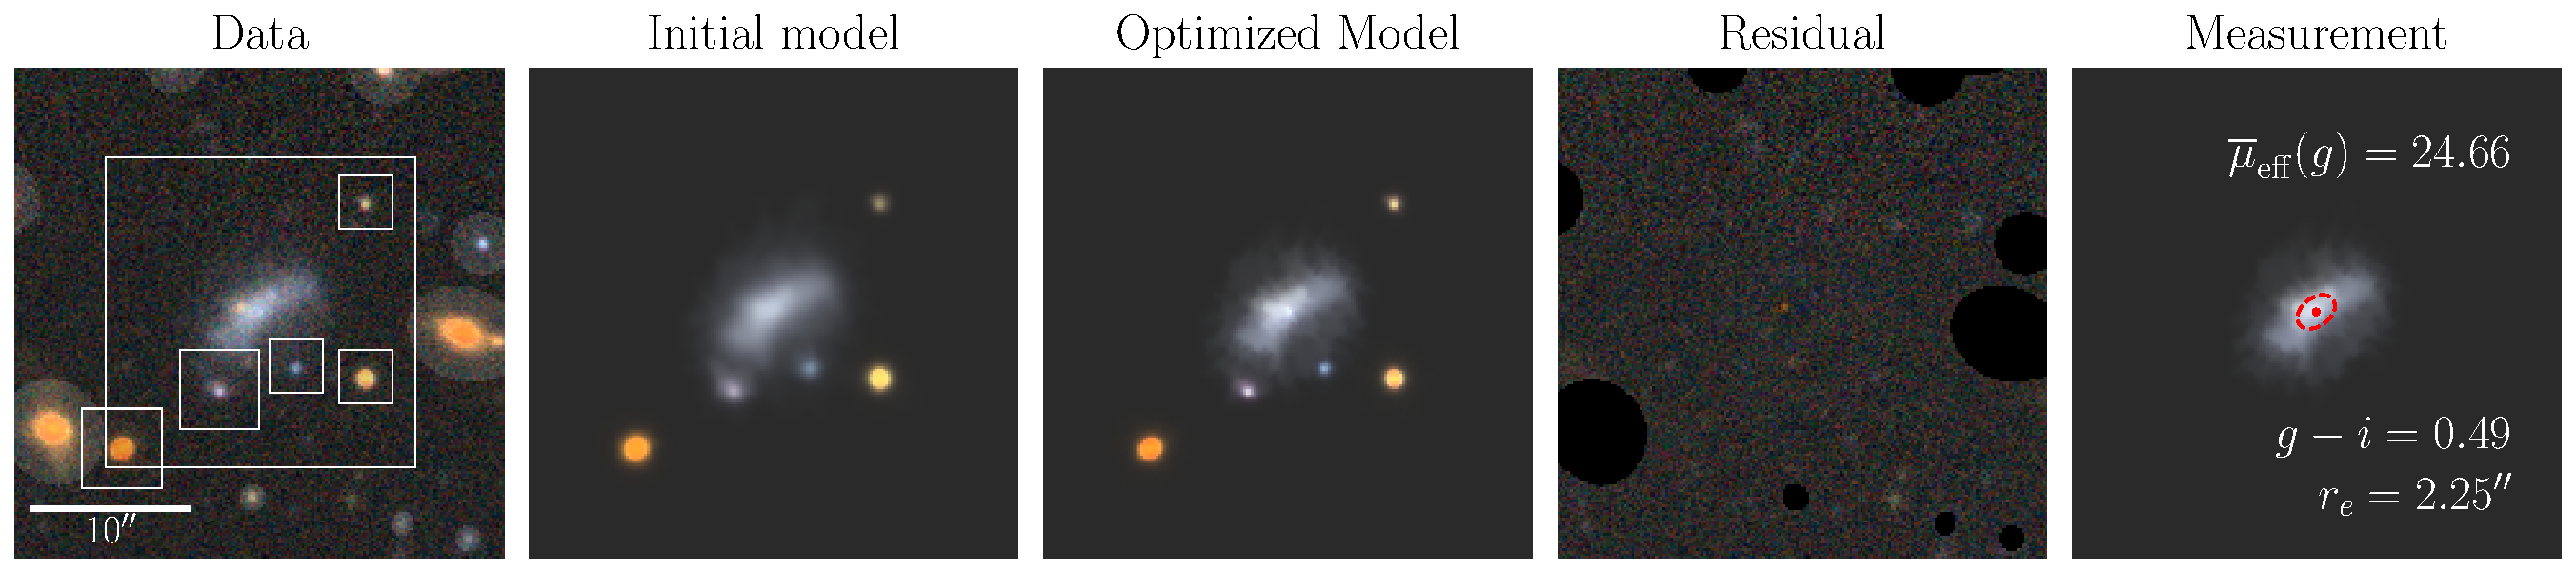
\includegraphics[width=1\linewidth]{vanilla_scarlet_demo.pdf}
		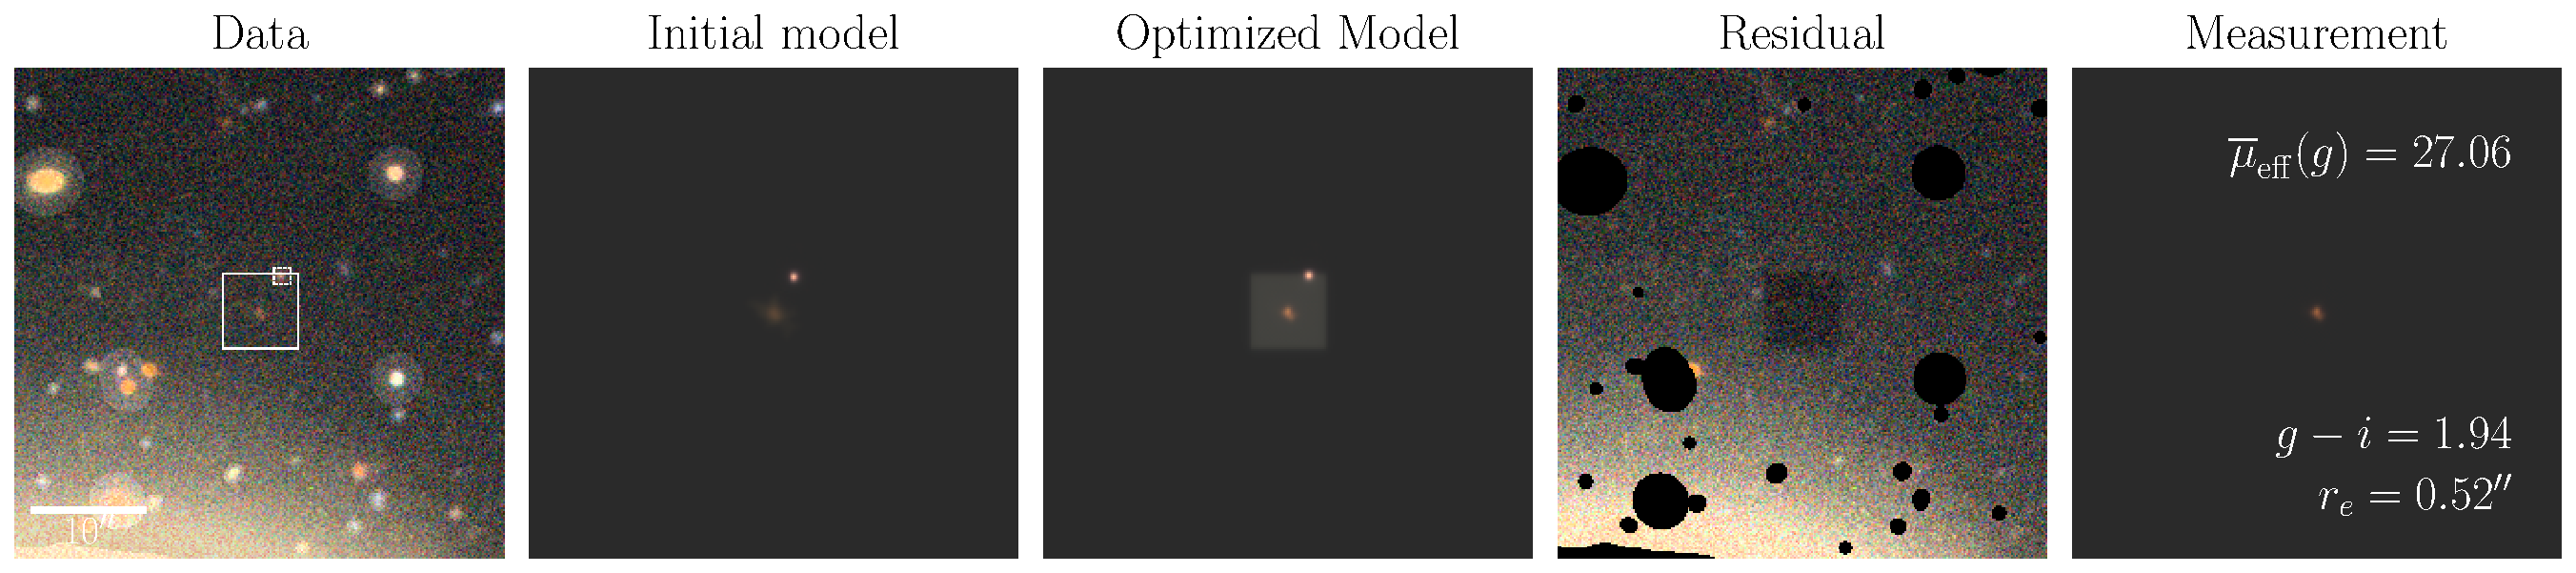
\includegraphics[width=1\linewidth]{vanilla_scarlet_demo2.pdf}
	}
	\caption{An example of the deblending step.}
	\label{fig:vanilla_scarlet_demo}
\end{figure*}

\end{enumerate}


Common false positives: why we want a deblending step
Why use scarlet: color info, non-par, monotonic, standard in future HSC, fast. Vanilla scarlet.
How does it work?



We design metric based on visual inspections for a random subset of LSBG candiates. 

We do not do scarlet fitting for the entire initial sample, because time consuming. We first match with MW hosts. 



\begin{figure*}
	\vbox{ 
		%\vskip -10mm
		\centering
		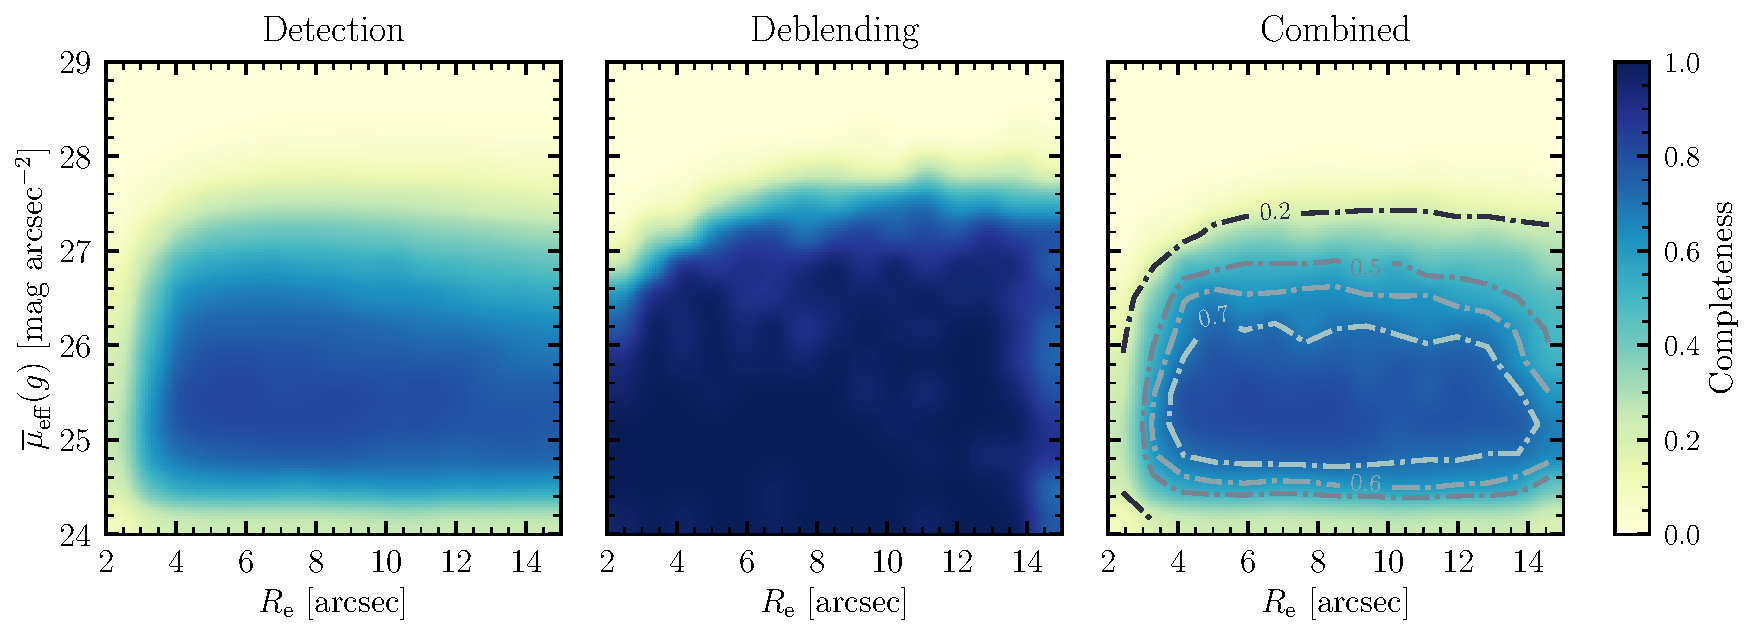
\includegraphics[width=1\linewidth]{completeness.pdf}
	}
	\caption{Caption}
	\label{fig:completeness}
\end{figure*}


\subsection{Completeness}

Since the scarlet model is PSF-deconvolved, the color is not affected by the seeing differences among bands. 


It is crucial to characterize the detection completeness in order to understand the intrinsic physical properties of the LSBG population. We performed a large suite of image simulation to derive the detection completeness. We inject $\sim 35,000$ mock galaxies with single \sersic{} light profiles \citep{Sersic1963} into the coadd images\footnote{We have also done extensive tests on injecting mock galaxies to the raw images and going through the entire data reduction pipeline. This is very expensive in terms of both CPU time and disk space, since we must run the full \code{hscPipe}. However, we find no noticable difference between this method and the direct injection to coadd images.}. The mock galaxies span a wide range in size ($2\arcsec \leqslant r_{e} \leqslant 21\arcsec$), surface brightness ($23 \leqslant \overline{\mu}_{\rm eff}(g) \leqslant 28.5\ \mathrm{mag\ arcsec^{-2}}$), \sersic{} index ($0.8 < n < 1.2$), and ellipticity ($0 < \epsilon < 0.6$) to match the LSBG distribution in \citetalias{Greco2018}. 

The detection completeness as a function of size and surface brightness is shown in the left panel of Figure \ref{fig:completeness}. The dependences of completeness on other parameters are very weak and are neglected in this work. The detection completeness falls steeply towards the high surface brightenss end and small end. This is because we manually excluded objects with high surface brightness in detection. 
\textbf{Explain it a little bit.}


\textbf{Wait... Is the detection efficiency map (jenny sent me) for S18A??? }


\subsection{Modeling and measurement error}




\section{UDGs in Milky-Way analogs}

\subsection{Matching with Milky-Way analogs}
The goal of this paper is to study the UDG population hosted by MW-like galaxies. However, the properties of MW itself vary in literature \citep{Licquia2015,Bland-Hawthorn2016}, and the definitions of MW analogs are also different among groups. In the SAGA survey \citep{SAGA-I,SAGA-II}, MW analogs are selected based on their absolute $K$-band magnitude $-23 > M_K > -24.6$, which is derived using abundance matching by assuming a simple galaxy-halo connection model (Fig 2 of \citealt{SAGA-I}). This luminosity range approximately corresponds to a stellar mass range of $10.2 < \log\, M_\star/M_\odot < 11.0$. They also require the MW analogs to be in isolation (without nearby bright galaxies) and lie in a redshift range of $0.005 < z < 0.01$ (20-40 Mpc). In the ELVES survey \citep{ELVES-I,ELVES-II,CarlstenELVES2022}, the requirements for MW-like host is loosened to be $M_K < -22.1$ ($M_\star > 10^{9.9}\ M_\odot$) because the probed volume by ELVES ($D<12$ Mpc) is smaller than that of SAGA. We choose the stellar mass range of MW analogs to be $10.2 < \log\, M_\star/M_\odot < 11.2$, which is simply a 1 dex bin centered at the measured stellar mass of the Milky Way ($\sim 10^{10.7}\ M_\odot$, \citealt{Licquia2015}). MW analogs selected using this definition is very close to those in SAGA but are slightly more massive than the ELVES hosts.

Since UDGs are relatively scarce in MW-like hosts \citep{SAGA-II,CarlstenELVES2022}, it is helpful to probe a larger volume to obtain good statistics. However, UDGs will be too small and faint to be detected in HSC images beyond certain distances. We choose our redshift range to be $0.01 < z < 0.04$, which makes sure that we can detect a significant number of faint dwarf galaxies around MW-like hosts. We exclude galaxies $z<0.01$ because 1) the number is very small; 2) their large angular size makes them shredded in deblending step, including them will introduce a lot of spurious LSB objects. Our MW analogs sample complements the ELVES sample and SAGA sample in redshift range. 

After applying the stellar mass and redshift cuts to the NSA catalog, there are 23,218 galaxies left. Then we match them to the LSBG catalog (described in Section \ref{subsec:detection}) as follows. For a given MW-like host, we first calculate its virial radius $R_{\rm vir}$ assuming the stellar mass-halo mass relation in \citet{Behroozi2010}. It turns out that 40\% of hosts have virial radii larger than 300 kpc. Then we identify any LSBG that falls into the projected angular virial radius of the host. Then these LSBGs are associated with the host. We repeat this process for all hosts. If one LSBG is associated to multiple hosts, we assign it to the nearest host (normalized by the angular size of virial radius). In the end, we have 901 MW-like hosts and 8,367 LSBG candidates associated with them. However, there are still a significant fraction of spurious objects in this LSBG sample, including galactic cirrus, tidal tails/streams, shrreded large galaxies, compact sources in galaxy outskirts, etc. In the following, we perform a deblending step to effectively remove these spurious objects. 

\subsection{UDG sample}
Remember to filter the UDG sample through the FDFC mask, and also remove duplicated objects.
\begin{figure}
    \centering
    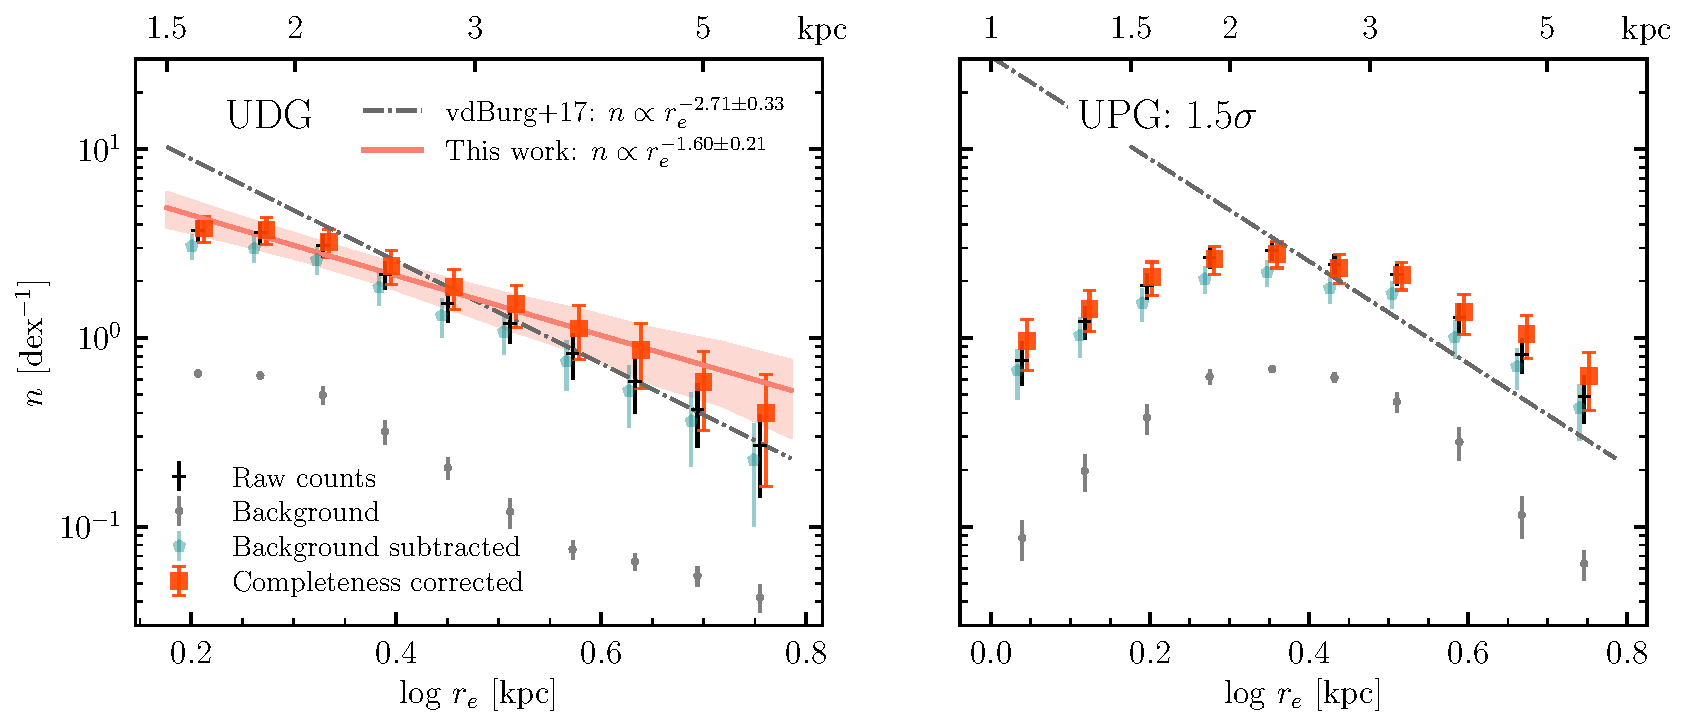
\includegraphics[width=1\linewidth]{size_distribution.pdf}
    \caption{Caption}
    \label{fig:size_distribution}
\end{figure}

\subsection{Spatial distribution}

\subsection{Quenched fraction}


\section{Discussion and Conclusion}
Scenarios:
1. violent environmental effects: radial orbits, back-splash both explain large size and quenching. But according to Bernavidis et al, the quenched fraction drops with increasing mass. 

2. accreting field UDGs, and quench them due to ram pressure stripping. But how long do accreted UDGs last before being destroyed? Need to look at ram pressure stripping literature.

Homework:
1. 1-sigma definition, UPG
2. number of UDG per host, as a function of host mass bins.
3. Move the stellar mass bin definition, try to match with red/blue, spiral/elliptical plot. If cannot match, does this hint the formation scenarios?
4. How significant do we detect blue UDGs? 
5. Split into redshift bins



TODO:
1. rerun the matching, compensate the left ~1000 LSBGs.
2. galactic extinction.

UDG rejuvenate after ram pressure stripping?


Why red is equivalent to quenched? Need to clarify in the paper

calculate probability of being a backsplash satellite (e.g., splashed to 1.5 Mpc)

Compare spatial distribution with normal dwarf? iF they are indeed high-spin tail of normal dwarfs. 

\section*{Acknowledgment}
JL is grateful for discussions with XXX.

\software{\href{http://www.numpy.org}{\code{NumPy}} \citep{Numpy},
          \href{https://www.astropy.org/}{\code{Astropy}} \citep{astropy},  \href{https://www.scipy.org}{\code{SciPy}} \citep{scipy}, \href{https://matplotlib.org}{\code{Matplotlib}} \citep{matplotlib},
          \href{https://halotools.readthedocs.io/en/latest}{\code{Halotools}} \citep{Hearin2017},
          \href{https://pmelchior.github.io/scarlet/}{\code{scarlet}} \citep{Melchior2018}
          }


\bibliography{citation}{}
\bibliographystyle{aasjournal}



\newpage
\appendix 

\section{Mock galaxy tests}

vdB 16 doesn't consider whether GALFIT gives the corrrect $R_e$, when deriving the completeness (recovered fraction)

\subsection{Spergel profile}

\subsection{\code{scarlet} measurement error}

\begin{figure}
    \centering
    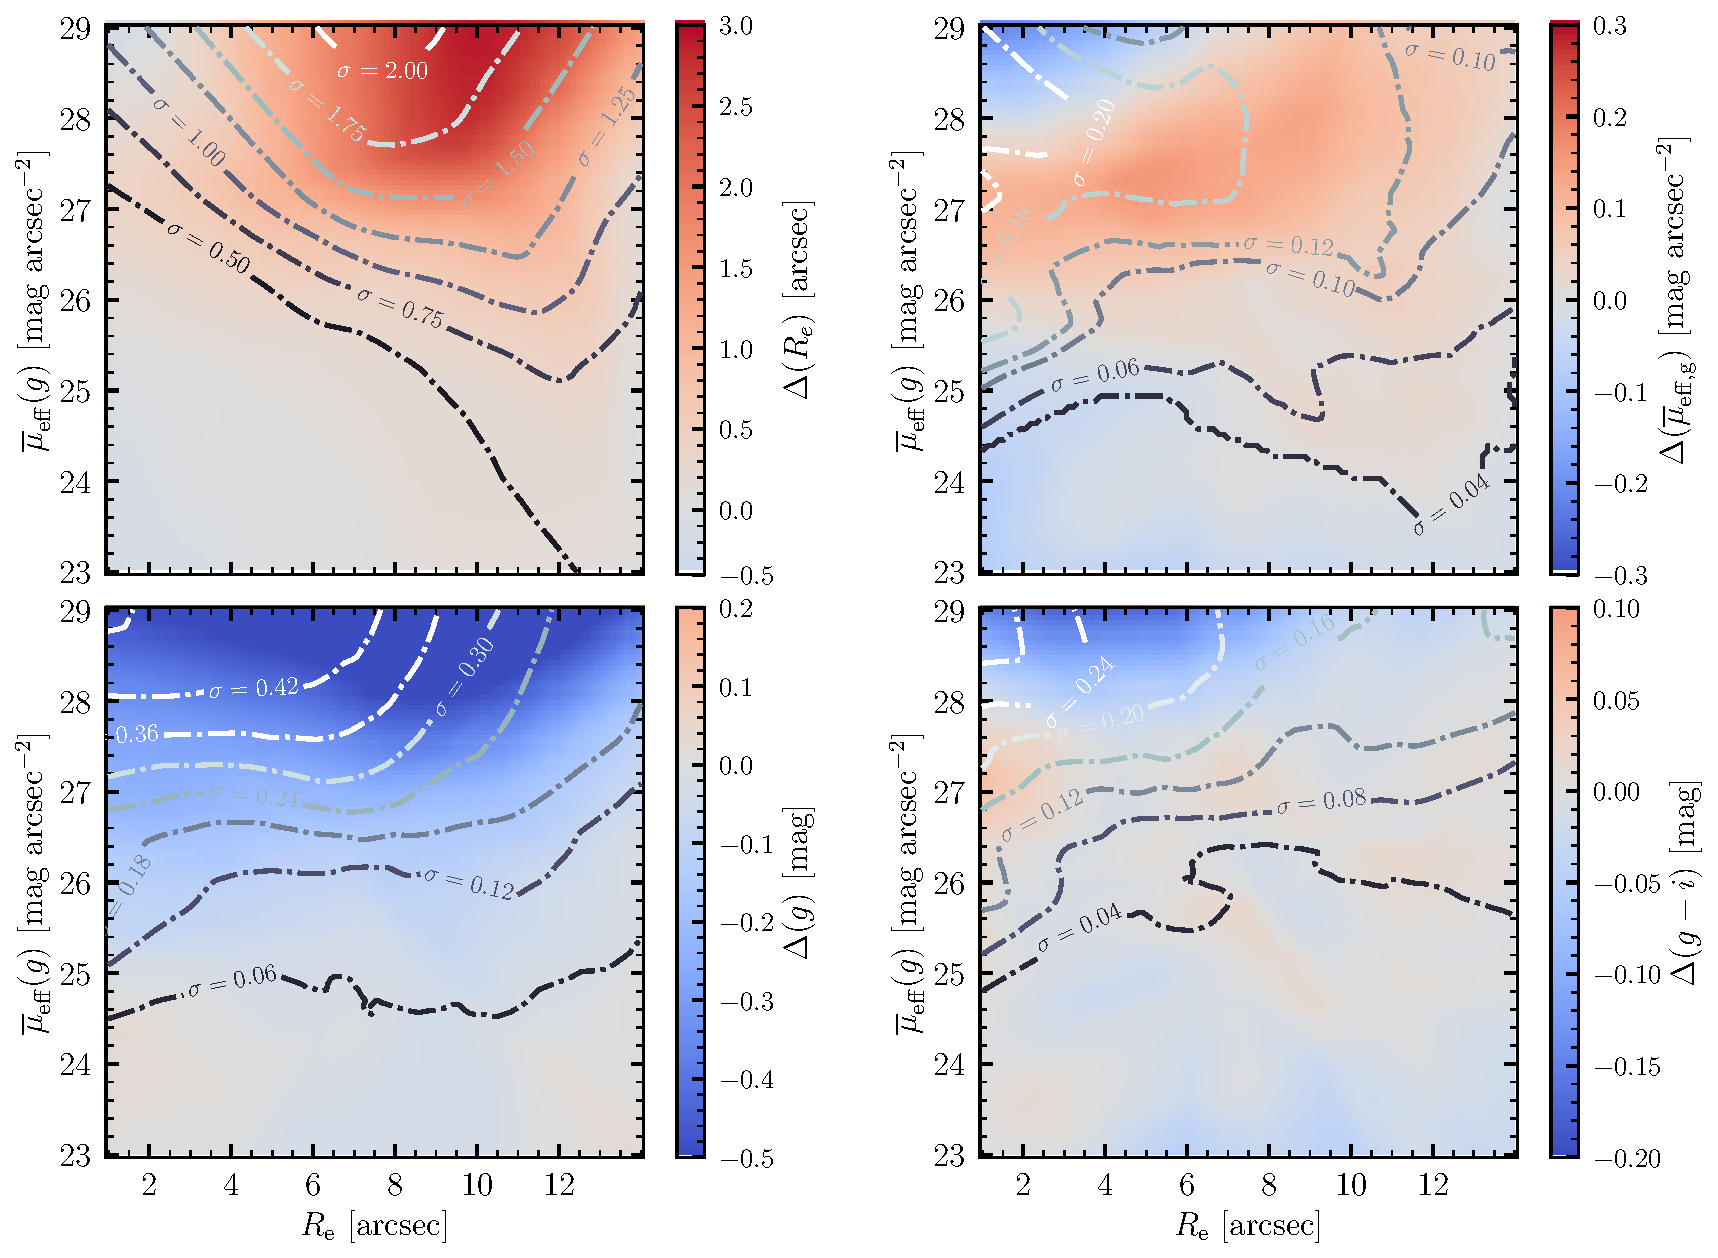
\includegraphics[width=1\linewidth]{meas_error_spergel.pdf}
    \caption{Caption}
    \label{fig:meas_err}
\end{figure}


%% This command is needed to show the entire author+affiliation list when
%% the collaboration and author truncation commands are used.  It has to
%% go at the end of the manuscript.
%\allauthors

%% Include this line if you are using the \added, \replaced, \deleted
%% commands to see a summary list of all changes at the end of the article.
%\listofchanges
\end{CJK*}
\end{document}

% End of file `sample631.tex'.
